\paragraph{Gene-gene co-occurrence network}
\label{section:gBg}

We post-processed the \egrine~ensemble to refine the underlying
network structure and discover functionally meaningful gene
co-regulatory modules present in the model. To do so, we transformed
the ensemble of biclusters into a weighted gene-gene association graph
$G$, where the nodes of $G$ are genes and the weight of edges between the
nodes is proportional to their frequency of co-occurrence in
biclusters:

\begin{equation}
w_{ij} = \frac{\left|B_i\cap B_j\right|}{\mathrm{min}(B_i,B_j)},
\end{equation}

\noindent where $w_{ij}$ is the weight of the edge between genes $i$ and $j$,
$B_i$ is the set of all biclusters containing gene $i$. The weights
were normalized by the minimum number of biclusters containing either
gene, rather than by the more typically applied union (which would
make the score identical to the Jaccard Index) to avoid penalizing
genes that occur infrequently in biclusters. The sum of edge weights
for each gene was normalized to one. This gene-gene co-occurrence
network represents how often \cm~ discovers co-regulation between
every pair of genes in the genome. We note that since this network is
derived from biclusters, it is also a reflection of conditional
co-expression and predicted \textit{cis}-­regulatory motifs.

\paragraph{Network backbone extraction}

After transforming the ensemble into a normalized graph, we removed
edges that were statistically indistinguishable by multiscale backbone
extraction (null hypothesis of uniform edge weight distribution given
a node of degree $k$) \cite{Serrano2009}. We retained all edges
satisfying the following relation:

\begin{equation}
\alpha_{ij}=1-(k-1)\int_0^{w_{ij}}(1-x)^{k-2}dx\leq 0.05,
\end{equation}

\noindent where $\alpha_{ij}$ is the probability that the normalized weight $w_{ij}$ between
genes $i$ and $j$ is compatible with the null hypothesis, and $k$ is
the degree of gene $i$. For \halo, backbone extraction reduced the
number of regulatory edges from 1,576,643 to 141,667; in \eco~ the
number of edges was reduced from 3,094,954 to 170,723.

\paragraph{Network link-community detection}
\label{section:linkcommunity}
Following backbone extraction, we detected corems by application of a
recently described link-community detection
algorithm \cite{Ahn2010}. For this algorithm to work on our data set
we modified it to accept input of a weighted graph \cite{Kalinka2011}.
We implemented it in \tmsamp{C++} for efficiency. The algorithm
computes a similarity score between all pairs of edges sharing a
common keystone node, $k$, according to the Tanimoto coefficient, $T$:

\begin{equation}
T(e_{ik},e_{kj}) = \frac{a_i\cdot a_j}{|a_i|^2+|a_i|^2+a_i\cdot a_j},
\end{equation}

\noindent where

\begin{equation}
a_i=w_{ij}+\frac{\delta_{ij}}{k_i}\sum_{l\in n(i)}w_{il}.
\end{equation}

\noindent Here, $e_{ik}$ is the edge between gene $i$
and the keystone gene $k$, and $\delta_{ij}$ is the Kroenecker delta. The score
reflects the similarity of gene neighborhoods adjacent to two edges
sharing a gene, with the score increasing in value as the number and
weight of overlapping adjacent edges increases. To transform the
Tanimoto coefficient into a distance metric, we compute $1-T$.

Following scoring, the edges were aggregated by standard hierarchical
clustering. The resulting tree is cut at many thresholds to optimize
the local weighted density $D$ of the resulting clusters:

\begin{equation}
D=\frac{1}{M\langle w\rangle}\sum_{c\in C}m_c\langle w\rangle_c\left(\frac{m_c-(n_c-1)}{n_c(n_c-1)/2-(n_c-1)}\right),
\end{equation}

\noindent where $M$ is the total number of edges in the
entire network, $\langle w\rangle$ is the average weight of edges in the entire
network, $C$ is the set of all link communities at a given threshold, $m_c$
is the number of edges in community $c$, $\langle w\rangle_c$ is the average weight of
edges in community $c$, and $n_c$ is the number of genes in community
$c$. The density scoring metric $D$ had a clear optimum corresponding exactly to
the cutoff that would have been chosen had we used the unweighted
scoring metric originally described (Figure \ref{fig:corem_density}). Only
communities with more than two genes were retained.

\begin{figure}[hp]
\centering
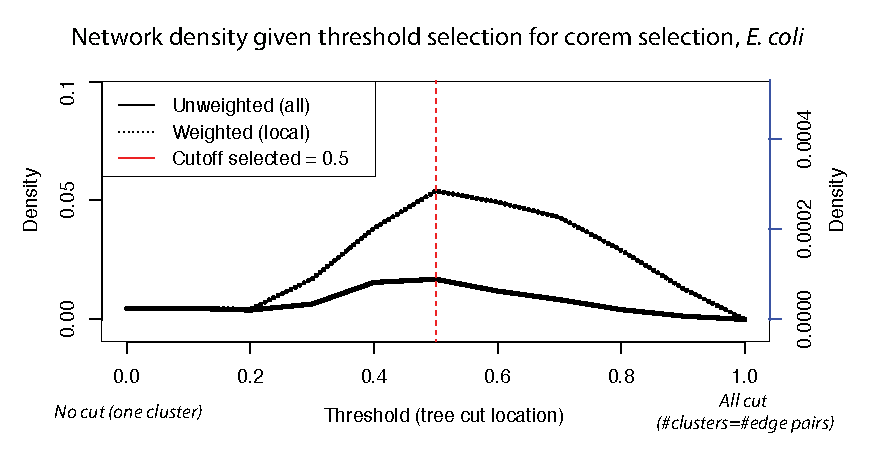
\includegraphics[width=0.9\linewidth]{figures/corem_density.pdf}
\caption[Corem density as a function of clustering cutoff threshold]{
{\bf Corem density as a function of clustering cutoff threshold.}
Hierarchical clustering cut threshold chosen to maximize the density
of resulting clusters. The cutoff chosen with modified weighted
density metric is identical to unweighted density metric.}
\label{fig:corem_density}
\end{figure}

Since the communities produced by this algorithm are comprised of sets
of edges, we defined a corem to include all genes incident to the
edges in a community. Because of this definition, each gene can be a
member of multiple different corems. In {\it H. salinarum}, this
procedure generated 679 corems ranging in size from 3 to 377 genes,
covering 1,363 of the 2,400 genes in the genome, and comprising 56,738
co-regulatory associations. In {\it E. coli}, we discovered 590
corems, ranging in size from 3 to 153 genes, covering 1,572 of 4,213
genes and 25,976 regulatory edges. See Table E1 and
Figure \ref{fig:corem_density} for additional
statistics. Gene-to-corem and corem-to-gene mappings for the {\it
H. salinarum} and {\it E. coli} models are available online.

\begin{figure}[hp]
\centering
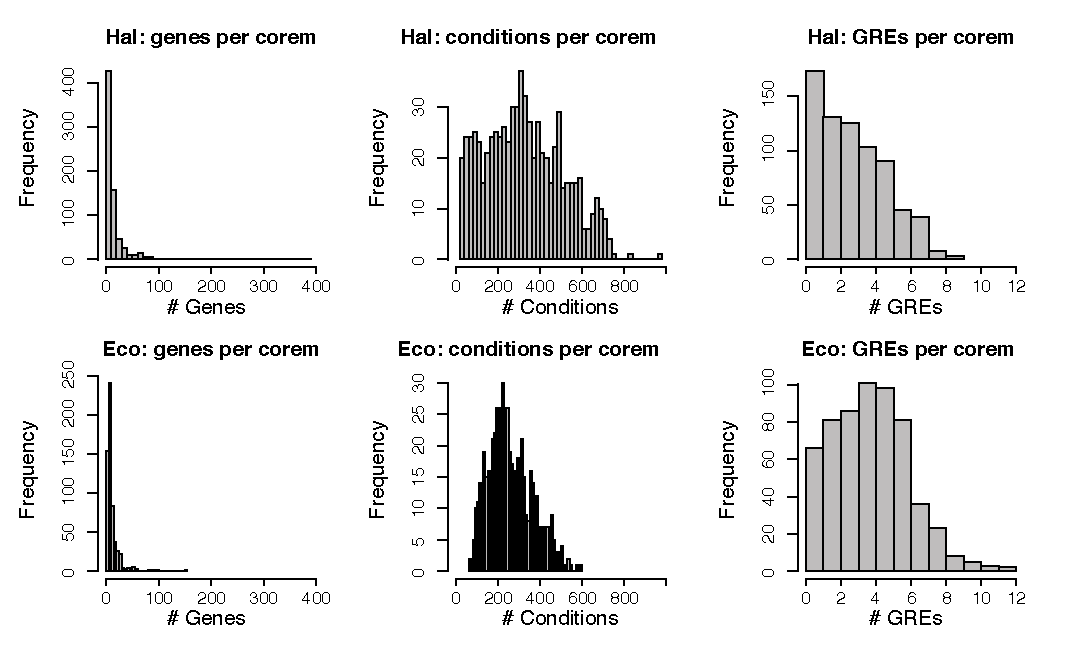
\includegraphics[width=0.9\linewidth]{figures/corem_stats.pdf}
\caption[Corem statistics]{
{\bf Corem statistics.} Number of genes, conditions, and GREs per
corem for \textit{E. coli} and \textit{H. salinarum} \egrine~models.}
\label{fig:corem_stats}
\end{figure}
